% move all configuration stuff into one file so we can focus on the content
\documentclass[aspectratio=169,hyperref={pdfpagelabels=false,colorlinks=true,linkcolor=white,urlcolor=blue},t]{beamer}

%%%%%%%%%%%%%%%%%%%%%%%%%%%%%%%%%%%%%%%%%%%%%%%%%%%%%%%%%%%%%%%%%%%%%%%%%%%%%%%%%%
%%%%%%%%%%%%%%%%%%%%%%%%%%%%%%%%%%%%%%%%%%%%%%%%%%%%%%%%%%%%%%%%%%%%%%%%%%%%%%%%%%
% packages
\usepackage{pict2e}
\usepackage{epic}
\usepackage{amsmath,amsfonts,amssymb}
\usepackage{units}
\usepackage{fancybox}
\usepackage[absolute,overlay]{textpos} 
\usepackage{media9} % avi2flv: "C:\Program Files\ffmpeg\bin\ffmpeg.exe" -i TuneFreqFilterbank.avi -b 600k -s 441x324 -r 15 -acodec copy TuneFreqFilterbank.flv
\usepackage{animate}
\usepackage{gensymb}
\usepackage{multirow}
\usepackage{silence}
\usepackage[backend=bibtex,style=ieee]{biblatex}
\AtEveryCitekey{\iffootnote{\tiny}{}}
\addbibresource{references}

%%%%%%%%%%%%%%%%%%%%%%%%%%%%%%%%%%%%%%%%%%%%%%%%%%%%%%%%%%%%%%%%%%%%%%%%%%%%%%%%%%
%%%%%%%%%%%%%%%%%%%%%%%%%%%%%%%%%%%%%%%%%%%%%%%%%%%%%%%%%%%%%%%%%%%%%%%%%%%%%%%%%%
% relative paths
\graphicspath{{graph/}}


%%%%%%%%%%%%%%%%%%%%%%%%%%%%%%%%%%%%%%%%%%%%%%%%%%%%%%%%%%%%%%%%%%%%%%%%%%%%%%%%%%
%%%%%%%%%%%%%%%%%%%%%%%%%%%%%%%%%%%%%%%%%%%%%%%%%%%%%%%%%%%%%%%%%%%%%%%%%%%%%%%%%%
% units
\setlength{\unitlength}{1mm}

%%%%%%%%%%%%%%%%%%%%%%%%%%%%%%%%%%%%%%%%%%%%%%%%%%%%%%%%%%%%%%%%%%%%%%%%%%%%%%%%%%
%%%%%%%%%%%%%%%%%%%%%%%%%%%%%%%%%%%%%%%%%%%%%%%%%%%%%%%%%%%%%%%%%%%%%%%%%%%%%%%%%%
% theme & layout
\usetheme{Frankfurt}
\beamertemplatenavigationsymbolsempty
%\setbeamertemplate{frametitle}[smoothbars theme]
\setbeamertemplate{frametitle}
{
    \begin{beamercolorbox}[ht=1.8em,wd=\paperwidth]{frametitle}
        \vspace{-.1em}%
        \hspace{.2em}{\strut\insertframetitle\strut}
        
        \hspace{.2em}\small\strut\insertframesubtitle\strut
        %\hfill
        %
\includegraphics[height=.8cm,keepaspectratio]{CenterMusicTechnology-solid-2lines-white-CoAtag}
        
    \end{beamercolorbox}
    \begin{textblock*}{100mm}(11.6cm,.7cm)
        \includegraphics[height=.8cm,keepaspectratio]{logo_GTCMT_black}
    \end{textblock*}
}

% set this to ensure bulletpoints without subsections
\usepackage{remreset}
\makeatletter
\@removefromreset{subsection}{section}
\makeatother
\setcounter{subsection}{1}

%---------------------------------------------------------------------------------
% appearance
\setbeamercolor{structure}{fg=gtgold}
\setbeamercovered{transparent} %invisible
\setbeamercolor{bibliography entry author}{fg=black}
\setbeamercolor*{bibliography entry title}{fg=black}
\setbeamercolor*{bibliography entry note}{fg=black}

%\usepackage{pgfpages}
%\setbeameroption{show notes}
%\setbeameroption{show notes on second screen=right}
%---------------------------------------------------------------------------------
% fontsize
\let\Tiny=\tiny

%%%%%%%%%%%%%%%%%%%%%%%%%%%%%%%%%%%%%%%%%%%%%%%%%%%%%%%%%%%%%%%%%%%%%%%%%%%%%%%%%%
%%%%%%%%%%%%%%%%%%%%%%%%%%%%%%%%%%%%%%%%%%%%%%%%%%%%%%%%%%%%%%%%%%%%%%%%%%%%%%%%%%
% warnings
\pdfsuppresswarningpagegroup=1
\WarningFilter{biblatex}{Patching footnotes failed}
\WarningFilter{latexfont}{Font shape}
\WarningFilter{latexfont}{Some font shapes}
\WarningFilter{gensymb}{Not defining}



\subtitle{Part 6.5: Tuning Frequency Estimation}

%%%%%%%%%%%%%%%%%%%%%%%%%%%%%%%%%%%%%%%%%%%%%%%%%%%%%%%%%%%%%%%%%%%%%%%%%%%%
\begin{document}
    % generate title page
	

\begin{frame}
    \titlepage
    %\vspace{-5mm}
    \begin{flushright}
        \href{http://www.gtcmt.gatech.edu}{\includegraphics[height=.8cm,keepaspectratio]{logo_GTCMT_black}}
    \end{flushright}
\end{frame}


    \section[overview]{lecture overview}
        \begin{frame}{tuning frequency}{overview}
            \begin{itemize}
                \item   \textbf{text book}  
                    \begin{itemize}
                        \item   \href{http://ieeexplore.ieee.org/xpl/articleDetails.jsp?tp=&arnumber=6331122&}{\underline{\textit{Chapter 5: Tonal Analysis} (pp.~88--90)}}
                        \item   \href{http://ieeexplore.ieee.org/xpl/articleDetails.jsp?tp=&arnumber=6331122&}{\underline{\textit{Chapter 5: Tonal Analysis} (pp.~106--108)}}
                    \end{itemize}
                \bigskip
                \item<2->   \textbf{lecture content}
                    \begin{itemize}
                        \item<2->   tuning frequency detection in polyphonic signals
                            \begin{itemize}
                                \item   problem description
                                \item   summary general approaches
                            \end{itemize}
                    \end{itemize}
            \end{itemize}
        \end{frame}

    \section[intro]{introduction}
        \begin{frame}{tuning frequency}{introduction 1/2}
            \begin{itemize}
                \item	\textit{frequency of concert pitch} $A4$
                \item	used to tune groups of instruments
                \item	standardized: \unit[440]{Hz}
            \end{itemize}
            \pause
            \vspace{3mm}
            \begin{itemize}
                \item	\textit{historic} tuning frequencies
                        \begin{footnotesize}\begin{table}
                            \vspace{-3mm}
                            %\centering
                            \begin{tabular}{lcc} %{c|p{12mm}p{12mm}p{12mm}p{12mm}p{12mm}p{12mm}p{12mm}}
                                \\ \hline
                                \bf{\emph{Year}}	 & \bf{\emph{Lower Deviation}}	 & \bf{\emph{Upper Deviation}}\\ 
                                 \hline
                                \bf{1750}	 & $-\unit[50]{Hz}$	 & $+\unit[30]{Hz}$\\
                                \bf{1850}	 & $-\unit[20]{Hz}$	 & $+\unit[20]{Hz}$\\
                                \bf{1950}	 & $-\unit[5]{Hz}$	 & $+\unit[10]{Hz}$\\
                            \end{tabular}
                        \end{table}\end{footnotesize}
            \end{itemize}
        \end{frame}
        
        \begin{frame}{tuning frequency}{introduction 2/2}
            \figwithmatlab{TuningFreqDistribution}
            \begin{itemize}
                \item	tuning frequencies \textit{today}
                        \begin{itemize}
                            \item	electronic music: \unit[440]{Hz}
                            \item	``classical'' music: (CSO, NYP: \unit[442]{Hz}; BP, VP: \unit[443]{Hz})
                        \end{itemize}
            \end{itemize}
        \end{frame}
        
        \begin{frame}{tuning frequency}{problem statement}
            \begin{itemize}
                \item   every pitch based analysis system relies on a tuning frequency standard
                \item   for (acoustic) recordings, the tuning frequency can largely vary
                \item   the temperament is unknown
                \item   expressive intonation is unknown
                
                \bigskip
                
                \item[$\Rightarrow$]<2->   a wrong tuning frequency assumption may impact the pitch reliability
            \end{itemize}
        \end{frame}

    \section[detection]{detection}
        \begin{frame}{tuning frequency}{brainstorm}
            \question{what are your ideas for detecting the tuning frequency in a complex mixture}
        \end{frame}
	\begin{frame}{tuning frequency estimation}{introduction}
		\begin{itemize}
			\item	\textbf{signal properties}
                \begin{itemize}
                    \item   not every signal/song contains A4 as a pitch
                    \item   the temperament is unknown
                    \item   expressive intonation is unknown
                \end{itemize}
                
            \bigskip
            \item<2->   \textbf{typical processing steps}
                \begin{enumerate}
                    \item<2->   estimate fundamental frequencies
                    
                    \item<3->   calculate deviation  $\Delta C$ from the nearest (equally tempered) pitch frequency in Cents
                    
                    \item<4->   average all deviations:  $\rightarrow \Delta \bar{C}$ 
                    
                    \item<5->   compute the tuning frequency from the average distance:
                        \begin{equation*}
                            \hat{f}_{A4} = \unit[440]{Hz} \cdot 2^\frac{\Delta \bar{C}}{1200}
                        \end{equation*}
                \end{enumerate}
		\end{itemize}
	\end{frame}
	\begin{frame}{tuning frequency estimation}{score-based}
		\begin{enumerate}
			\item	analyze score and \textbf{identify important pitches}
			\item<2->	define a set of narrow \textbf{band pass filters} per pitch
			\item<3->	\textbf{sweep band pass} filter's  mid frequency over selected audio segments
			\item<4->	identify most likely \textbf{mid frequency} maximizing the filter's output energy 
            \item<5->  compute its \textbf{deviation} $\Delta C$ from the (equally tempered) pitch frequency in Cents
			\item<6->	\textbf{average} all results
			\item<7->	compute overall result in Hertz
		\end{enumerate}
	\end{frame}
	\begin{frame}{tuning frequency estimation}{STFT-based}
		\begin{enumerate}
			\item	identify \textbf{spectral peaks}
			\item<2->	compute \textbf{instantaneous frequencies} $f_\mathrm{I}(k)$
			\item<3->	compute \textbf{distance} to nearest equally tempered semitone frequency $\hat{f}_{A4}(n-1)$ (in Cents)
			\item<4->	iteratively \textbf{adjust tuning frequency} estimate to minimize distance
		\end{enumerate}
	\end{frame}
	\begin{frame}{tuning frequency estimation}{histogram-based}
		\begin{enumerate}
			\item	compute \textbf{CQT}: bin resolution \unit[10]{Cents}
			\item<2->	compute \textbf{distance} of peaks to nearest equally tempered semitone frequency @ $f_{A4}=\unit[440]{Hz}$ (in Cents)
			\item<3->	compute \textbf{histogram of deviations}
			\item<4->	choose \textbf{position of histogram maximum} as tuning frequency deviation from $f_{A4}$
		\end{enumerate}
	\end{frame}
	\begin{frame}{tuning frequency estimation}{filterbank-based 1/2}
    \vspace{-5mm}
        \begin{columns}
        \column{.5\textwidth}
            \begin{enumerate}
                \item	filterbank with 3 closely spaced filters per semi-tone
                \item<2->	compute output energy for every triplet $E_j(0,n),E_j(1,n),E_j(2,n)$
                \item<3->	compute overall triplet output energy 
                    \begin{equation*}
                        E(\cdot,n)	= \sum\limits_{\forall j}{E_j(\cdot,n)}
                    \end{equation*}

            \end{enumerate}
        \column{.5\textwidth}
            \only<1>{
            %\begin{figure}
                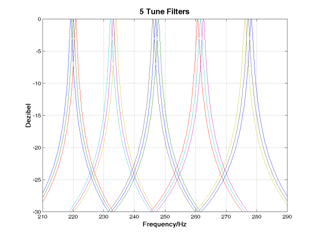
\includegraphics[scale=.5]{graph/tuningfreqfb}
            %\end{figure}
            }
            \only<3>{
            \begin{figure}
                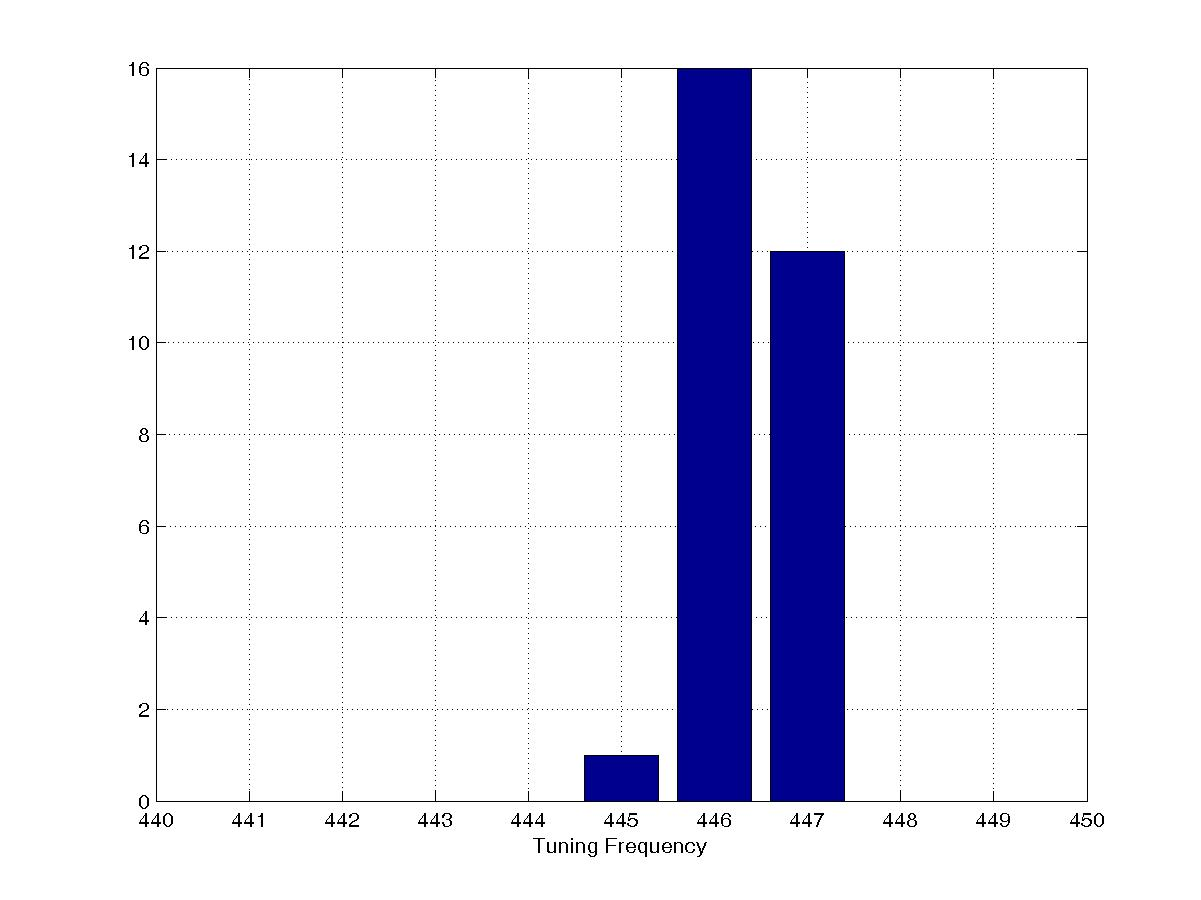
\includegraphics[scale=.125]{graph/tuningfreq_energy}
            \end{figure}
            }
        \end{columns}
        \begin{flushright}
            plots from \footfullcite{lerch_ansatz_2004},\footfullcite{lerch_requirement_2006}
        \end{flushright}
	\end{frame}
	\begin{frame}{tuning frequency estimation}{filterbank-based 2/2}
		\begin{enumerate}
			\setcounter{enumi}{3}
			\item	adapt current tuning frequency estimate
				\begin{equation*}
					\hat{f}_{A4}(n+1) = \big(1 + \sign\left(E(2)-E(0)\right)\cdot \lambda \big)\cdot \hat{f}_{A4}(n)
				\end{equation*}
				\vspace{-2mm}
				\begin{itemize}
					\item[] $\lambda$: scaled up if adaption direction remains, otherwise scaled down
				\end{itemize}
				\only<3>
                {
                    \vspace{-5mm}
                    \figwithmatlab{Rprop}
				}
				\only<4>{
                    \videowithmatlab{FilterbankAdaptation}
				}
		\end{enumerate}
        \vspace{30mm}
	\end{frame}            
   \section[summary]{lecture summary}
        \begin{frame}{summary}{lecture content}
            \begin{enumerate}
                \item    why can the tuning frequency be important for pitch-related analyses?
                \smallskip
                \item<2-> what is one of the basic assumptions for most detection algorithms presented here?
            \end{enumerate}
        \end{frame}
\end{document}

